\chapter{Khoảng cách riêng, hình học Kruskal và các quan sát viên ở chân trời}

Metric Schwarzschild dường như trở nên kỳ dị tại chân trời. Độ cong thì không. Để tách bạch hai mệnh đề đó, trước hết ta khử kích thước tổng thể của lỗ đen, rồi thay tọa độ xuyên tâm bằng khoảng cách riêng tính từ chân trời. Gần chân trời, hình học thu được là không-thời gian phẳng thông thường được viết trong các tọa độ gia tốc. Một khi hình học ấy đã được vẽ ra, các câu hỏi về Alice, Bob và Charlie trở thành các câu hỏi về đường thế giới và tia sáng, chứ không còn là những nghịch lý ngôn từ.

\section{Tách thang bán kính Schwarzschild}

Bắt đầu với các tọa độ có dấu phẩy để rồi các biến đã co giãn lại có thể mang những tên quen thuộc:
\begin{equation}
d\tau^2
=
\left(1-\frac{2MG}{r'}\right)dt'^2
-
\frac{dr'^2}{1-\frac{2MG}{r'}}
-
r'^2d\Omega_2^2.
\label{eq:l7-schwarzschild-dimensional}
\end{equation}
Đặt bán kính Schwarzschild và các tọa độ không thứ nguyên
\begin{equation}
r_{\mathrm S}=2MG,
\qquad
r=\frac{r'}{r_{\mathrm S}},
\qquad
t=\frac{t'}{r_{\mathrm S}}.
\label{eq:l7-rescaling}
\end{equation}
Ta lấy \(c=1\), nên thời gian và độ dài có cùng đơn vị. Vì vậy bán kính \(r_{\mathrm S}\) vừa là một độ dài vừa là thời gian để ánh sáng đi hết độ dài ấy. Thế vào, ta được
\begin{equation}
d\tau^2
=r_{\mathrm S}^2
\left[
\left(1-\frac1r\right)dt^2
-
\frac{dr^2}{1-\frac1r}
-
r^2d\Omega_2^2
\right].
\label{eq:l7-schwarzschild-rescaled}
\end{equation}
Do đó, mọi lỗ đen Schwarzschild không quay và không tích điện đều có cùng một hình học không thứ nguyên. Thay đổi khối lượng làm thay đổi thang đo nhân với metric, chứ không làm thay đổi dạng của biểu thức trong ngoặc vuông. Tình huống này giống như vẽ các mặt cầu sau khi chia mọi khoảng cách cho bán kính của cầu: cùng một hình vẽ mô tả Mặt Trăng và Trái Đất, mặc dù một xentimét trên mỗi hình vẽ biểu thị một khoảng cách vật lý khác nhau.

\begin{classroomqa}
\audiencequestion{Những dấu nào đi với các phần xuyên tâm và góc của metric?}
\lecturerresponse{Với chữ ký \(+---\) được dùng ở đây, cả hai phần không gian đều mang dấu trừ. Cả phòng đã nhận ra dấu ấy khi biểu thức đang được viết ra. Thừa số góc có thể dùng sine hoặc cosine tùy theo việc tọa độ cực được đo từ trục hay từ xích đạo; kí hiệu gọn \(d\Omega_2^2\) tránh được vấn đề quy ước đó.
\lecturetimestamp{00:07:48--00:08:12}}
\end{classroomqa}

\section{Thang độ cong tại chân trời}

Việc co giãn lại này trả lời một câu hỏi vật lý quan trọng mà không cần một phép tính tensor dài. Một thành phần của metric là không thứ nguyên. Một ký hiệu Christoffel chứa một đạo hàm theo tọa độ và vì thế có thứ nguyên nghịch đảo độ dài, trong khi một thành phần của tensor Riemann trong một cơ sở trực chuẩn vật lý có thứ nguyên
\begin{equation}
[g_{\mu\nu}]=1,
\qquad
[\Gamma^\mu{}_{\nu\rho}]=L^{-1},
\qquad
[R_{\hat\alpha\hat\beta\hat\gamma\hat\delta}]
=L^{-2}.
\label{eq:l7-curvature-dimensions}
\end{equation}
Tại chân trời \(r=1\), độ dài vật lý duy nhất sẵn có là
\(r_{\mathrm S}\). Vì vậy, thang độ cong thủy triều phải là
\begin{equation}
\left|R_{\hat\alpha\hat\beta\hat\gamma\hat\delta}\right|_{\mathrm{hor}}
\sim \frac{1}{r_{\mathrm S}^2}.
\label{eq:l7-horizon-curvature}
\end{equation}
Tổng quát hơn, nó là \(r_{\mathrm S}^{-2}\) nhân với một hàm không thứ nguyên của
\(r\). Mệnh đề này nói về trường thủy triều Riemann, không phải vô hướng Ricci, vốn triệt tiêu trong chân không Schwarzschild.

Kết luận vật lý rút ra ngay lập tức. Tăng khối lượng làm tăng
\(r_{\mathrm S}\) và làm yếu trường thủy triều tại chân trời. Một lỗ đen nhỏ có thể xé một vật có kích thước hữu hạn ra trong lúc nó băng qua; gần chân trời của một lỗ đen siêu khối lượng, lực thủy triều có thể nhẹ. Tuy nhiên, độ cong tăng lên khi đi vào trong và phân kỳ tại \(r=0\). Vì vậy, chân trời và điểm kỳ dị là hai đối tượng khác nhau một cách căn bản.

\section{Khoảng cách riêng tính từ chân trời}

Trong phần còn lại của phép tính cục bộ, đặt \(r_{\mathrm S}=1\). Trong thuyết tương đối, thay đổi tọa độ không chỉ là chuyện hình thức: một tọa độ tồi có thể che khuất một hình học chính quy sau các hệ số kỳ dị. Độ chênh tọa độ Schwarzschild \(r-1\) không phải là khoảng cách xuyên tâm đo được từ chân trời.

\begin{figure}[htbp]
\centering
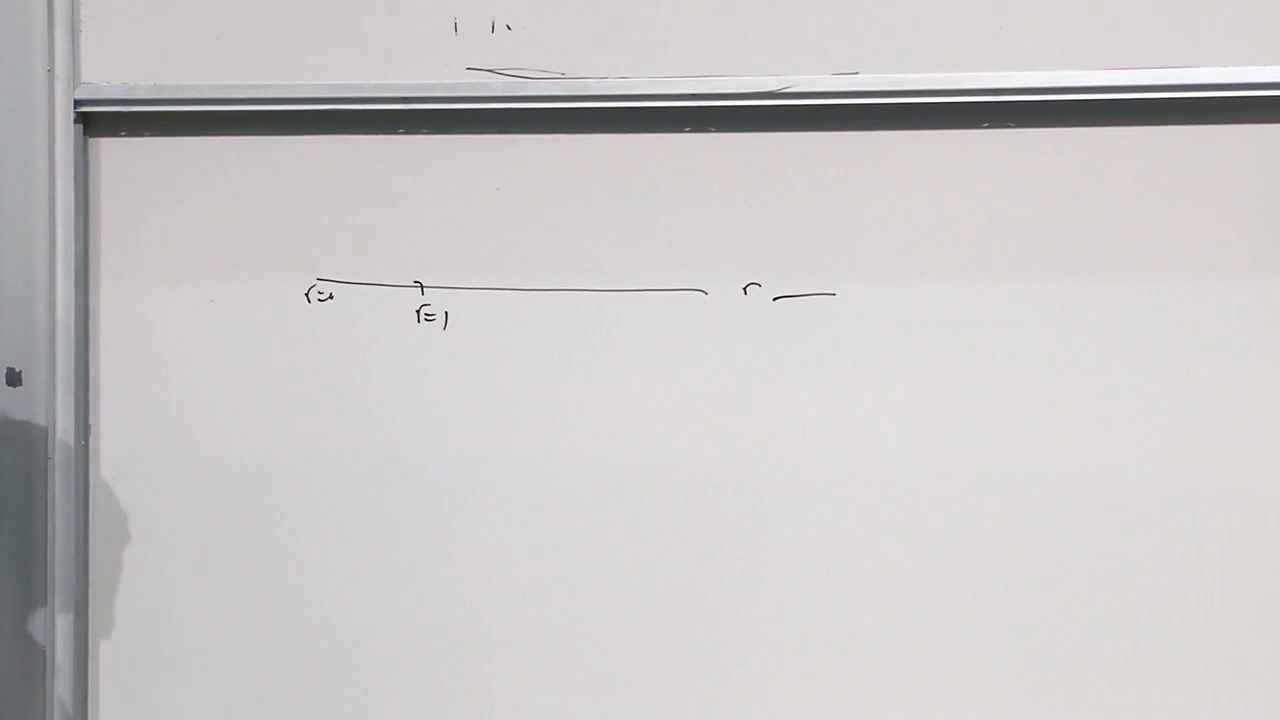
\includegraphics[width=0.78\textwidth]{lecture_07_figure_02.png}
\caption{Trục tọa độ xuyên tâm được dùng trên bảng. Chân trời ở
\(r=1\), còn \(r=0\) là điểm kỳ dị độ cong.}
\lectureframe{00:16:11}
\end{figure}

Giữ \(t\) và các góc cố định. Khi đó phần tử độ dài không gian dương là
\begin{equation}
ds^2=\frac{dr^2}{1-\frac1r},
\qquad
ds=\sqrt{\frac{r}{r-1}}\,dr.
\label{eq:l7-radial-proper-line}
\end{equation}
Định nghĩa khoảng cách riêng không thứ nguyên tính từ chân trời bởi
\begin{equation}
\rho(r)
=
\int_1^r\sqrt{\frac{r'}{r'-1}}\,dr'.
\label{eq:l7-rho-definition}
\end{equation}
Khoảng cách vật lý là \(r_{\mathrm S}\rho\) khi khôi phục lại thang tổng thể. Ta sẽ không cần dạng đóng của tích phân. Ta chỉ cần đạo hàm của nó:
\begin{equation}
\frac{d\rho}{dr}
=\sqrt{\frac{r}{r-1}},
\qquad
d\rho^2
=\frac{dr^2}{1-\frac1r}.
\label{eq:l7-rho-derivative}
\end{equation}
Vì vậy, hạng xuyên tâm phức tạp trở thành đúng bằng \(-d\rho^2\). Sự đơn giản hóa đó là lý do để đưa vào \(\rho\).

Bây giờ co giãn lại tọa độ thời gian thêm một lần nữa,
\begin{equation}
\omega=\frac{t}{2}.
\label{eq:l7-omega}
\end{equation}
Vì \(r\) là một hàm của \(\rho\), metric có thể được viết thành
\begin{equation}
d\tau^2
=
F(\rho)\rho^2d\omega^2
-
d\rho^2
-
r(\rho)^2d\Omega_2^2.
\label{eq:l7-rho-metric}
\end{equation}

\begin{classroomqa}
\audiencequestion{Có phải \(F(\rho)\) được định nghĩa đơn thuần để hệ số thời gian có dạng \(F(\rho)\rho^2\) hay không?}
\lecturerresponse{Đúng. Ở thời điểm này, phép tách nhân tử ấy không có nội dung vật lý độc lập nào. Đó là một định nghĩa thuận tiện. Tính hữu ích của nó xuất hiện khi lấy các giới hạn của \(F\) ở gần và xa chân trời.
\lecturetimestamp{00:26:39--00:26:59}}
\end{classroomqa}

Ở xa, hệ số thời gian của Schwarzschild tiến tới 1. Vì
\(dt=2d\omega\), điều này trở thành
\begin{equation}
\lim_{\rho\to\infty}F(\rho)\rho^2=4.
\label{eq:l7-far-limit}
\end{equation}
Gần chân trời, Phương trình~\eqref{eq:l7-rho-definition} cho
\begin{equation}
\begin{aligned}
\rho&\simeq 2\sqrt{r-1},\\
r(\rho)&=1+\frac{\rho^2}{4}+O(\rho^4),\\
\lim_{\rho\to0}F(\rho)&=1.
\end{aligned}
\label{eq:l7-near-expansion}
\end{equation}

\begin{figure}[htbp]
\centering
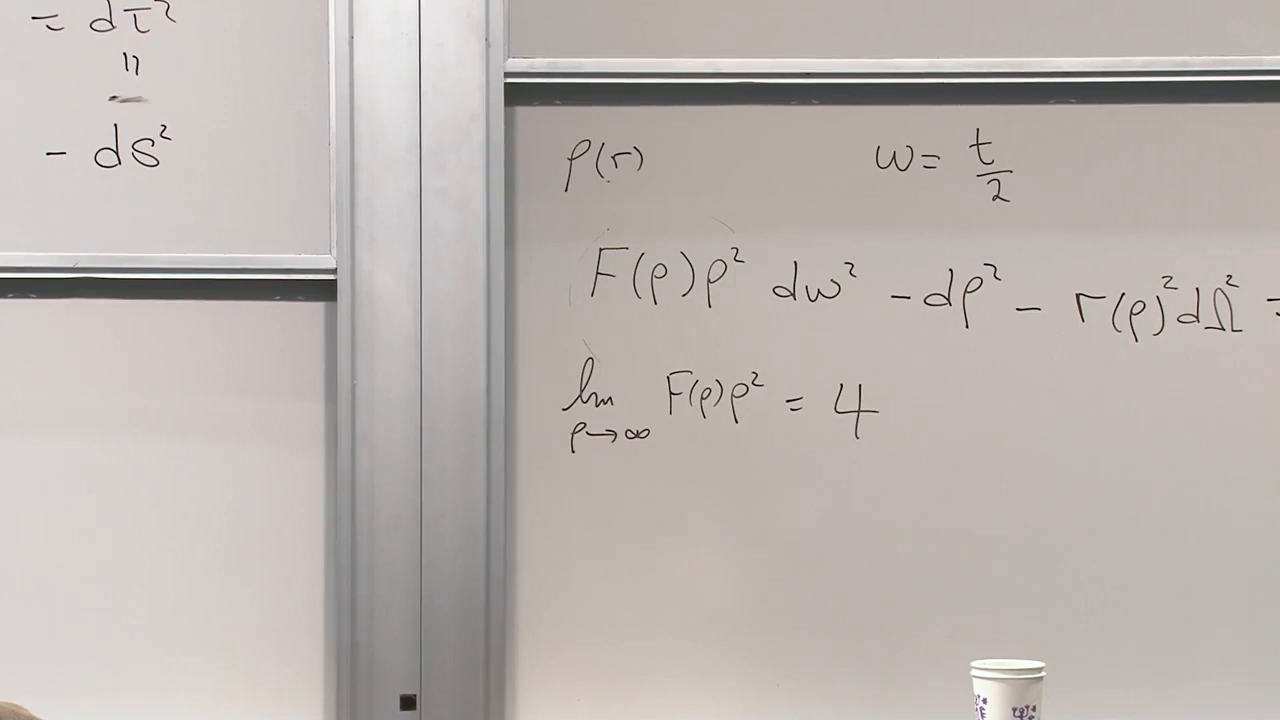
\includegraphics[width=0.90\textwidth]{lecture_07_figure_03.png}
\caption{Metric trong \((\rho,\omega)\), hệ số thời gian tiệm cận của nó, và các giới hạn gần chân trời \(F\to1\) và
\(r=1+\rho^2/4+\cdots\).}
\lectureframe{00:37:30}
\end{figure}

\section{Không-thời gian phẳng ẩn ở chân trời}

Gần \(\rho=0\), phần thời gian-xuyên tâm của
Phương trình~\eqref{eq:l7-rho-metric} rút gọn thành
\begin{equation}
d\tau_{\mathrm{radial}}^2
\simeq
\rho^2d\omega^2-d\rho^2.
\label{eq:l7-rindler-metric}
\end{equation}
Đây là không-thời gian Minkowski phẳng trong tọa độ cực hypebol. Định nghĩa
\begin{equation}
X=\rho\cosh\omega,
\qquad
T=\rho\sinh\omega.
\label{eq:l7-rindler-transform}
\end{equation}
Khi đó
\begin{equation}
dT^2-dX^2
=
\rho^2d\omega^2-d\rho^2.
\label{eq:l7-minkowski-check}
\end{equation}
Các đường \(\rho\) không đổi thỏa mãn
\begin{equation}
X^2-T^2=\rho^2
\label{eq:l7-constant-rho}
\end{equation}
và là các hypebol. Các đường \(\omega\) không đổi là các tia phát ra từ gốc tọa độ. Khi \(\omega\to\infty\), các tia ấy tiến gần đến đường null \(T=X\). Vì vậy, chân trời Schwarzschild, vốn dường như bị đẩy ra thời gian tọa độ vô hạn, thực ra chỉ là một đường null thông thường trong giản đồ chính quy.

\begin{figure}[htbp]
\centering
\includegraphics[width=0.88\textwidth]{lecture_07_figure_06.png}
\caption{Hình học hoàn chỉnh trên bảng: các hypebol \(\rho\) không đổi, các tia \(\omega\) không đổi, chân trời null, và miền \(r<1\) ở phía trên nó.}
\lectureframe{00:38:30}
\end{figure}

\begin{figure}[htbp]
\centering
\resizebox{0.96\linewidth}{!}{%
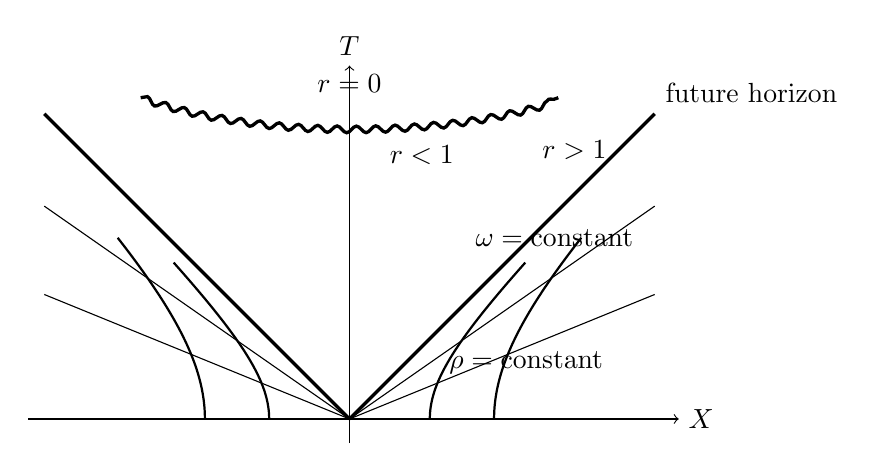
\begin{tikzpicture}[scale=1.02]
\draw[->] (-4.0,0) -- (4.1,0) node[right] {$X$};
\draw[->] (0,-0.3) -- (0,4.4) node[above] {$T$};
\draw[very thick] (0,0) -- (3.8,3.8)
  node[above right] {future horizon};
\draw[very thick] (0,0) -- (-3.8,3.8);
\draw[thick]
  plot[domain=0:1.42,samples=50]
  ({1.0*cosh(\x)},{1.0*sinh(\x)});
\draw[thick]
  plot[domain=0:1.05,samples=50]
  ({1.8*cosh(\x)},{1.8*sinh(\x)});
\draw[thick]
  plot[domain=0:1.42,samples=50]
  ({-1.0*cosh(\x)},{1.0*sinh(\x)});
\draw[thick]
  plot[domain=0:1.05,samples=50]
  ({-1.8*cosh(\x)},{1.8*sinh(\x)});
\draw[thin] (0,0) -- (3.8,1.55);
\draw[thin] (0,0) -- (3.8,2.65);
\draw[thin] (0,0) -- (-3.8,1.55);
\draw[thin] (0,0) -- (-3.8,2.65);
\draw[very thick,decorate,decoration={snake,amplitude=1.2pt,segment length=7pt}]
  (-2.6,4.0) .. controls (-1.2,3.5) and (1.2,3.5) .. (2.6,4.0);
\node at (0,4.18) {$r=0$};
\node at (2.2,0.7) {$\rho=\mathrm{constant}$};
\node at (2.55,2.25) {$\omega=\mathrm{constant}$};
\node at (0.9,3.28) {$r<1$};
\node at (2.8,3.35) {$r>1$};
\end{tikzpicture}
}
\caption{Một sự tái dựng nhân quả sáng sủa. Chân trời là một đường null, còn điểm kỳ dị độ cong \(r=0\) là một biên tương lai ở bên trong lỗ đen.}
\label{fig:l7-kruskal-clean}
\end{figure}

Giới hạn \(\rho\) nhỏ không giống giới hạn bán kính nhỏ trong tọa độ cực Euclid. Một đường tròn Euclid nhỏ co lại về một điểm. Một hypebol \(\rho\) không đổi tiến gần đến cả một đường null. Vì vậy \(\rho=0\) gắn nhãn cho toàn bộ chân trời, chứ không chỉ cho điểm giao nhau của các trục.

Công thức ở miền ngoài có thể được tiếp tục giải tích vào \(r<1\). Gần chân trời, \(r-1\simeq\rho^2/4\), nên miền trong về mặt hình thức tương ứng với
\(\rho^2<0\). Có thể gọi \(\rho\) là ảo, nhưng dùng \(\rho^2\), \(r\), hoặc các tọa độ chính quy \(T,X\) thì sáng sủa hơn. Ở bên trong, dấu của các hệ số Schwarzschild đi với \(t\) và \(r\) hoán đổi cho nhau. Điều đó không có nghĩa là một chiếc đồng hồ đeo tay vật lý biến thành một cây thước. Nó có nghĩa là các tọa độ Schwarzschild đã hoán đổi tính chất nhân quả của chúng.

\begin{classroomqa}
\audiencequestion{Các hypebol nằm ngang ở bên trong chân trời là gì, và các tia thẳng là gì?}
\lecturerresponse{Các đường hypebol là các đường \(r\) không đổi, hay tương đương là \(\rho^2\) không đổi, được tiếp tục vào \(r<1\). Các tia là các đường có thời gian Schwarzschild không đổi. Ở bên ngoài, chúng tạo thành một lưới tọa độ hữu ích; ở bên trong, không được nhầm các nhãn ấy với các quỹ đạo của quan sát viên vật lý.
\lecturetimestamp{00:44:12--00:44:59}}
\end{classroomqa}

\begin{classroomqa}
\audiencequestion{Phương thẳng đứng có phải là một tọa độ thời gian không, và nó biểu diễn hệ quy chiếu của ai?}
\lecturerresponse{Nó là một hướng thời gian chính quy trong giản đồ không-thời gian mới, nhưng không phải thời gian Schwarzschild kỳ dị \(t\). Giản đồ này thích nghi với cấu trúc nhân quả của rơi tự do. Một quan sát viên bị giữ ở bán kính ngoài cố định đi theo một hypebol và phải gia tốc; một quan sát viên rơi tự do đi qua chân trời null một cách trơn tru.
\lecturetimestamp{00:45:54--00:46:48}}
\end{classroomqa}

\begin{classroomqa}
\audiencequestion{Nếu \(\rho^2<0\) ở bên trong, thì thừa số \(i\) tường minh ở đâu?}
\lecturerresponse{Có thể đưa vào một \(\rho\) ảo, nhưng làm vậy không thu được gì. Nội dung bất biến nằm ở \(r\), ở \(\rho^2\), và ở các tọa độ chính quy thực \(T,X\). Hệ thức
\(r-1\simeq\rho^2/4\) chỉ là khai triển gần chân trời.
\lecturetimestamp{00:52:35--00:53:00}}
\end{classroomqa}

Giản đồ chính quy này thường được mô tả trong bài giảng như là bức tranh Kruskal. Nói nghiêm ngặt, các tọa độ Kruskal chính xác bao gồm một thừa số xuyên tâm giữ cho toàn bộ metric Schwarzschild là chính quy, trong khi Phương trình~\eqref{eq:l7-rindler-transform} là dạng gần chân trời của nó. Thông điệp nhân quả là như nhau: chân trời là trơn, nhưng mọi đường cong kiểu thời hoặc null hướng tương lai ở bên trong đều kết thúc tại \(r=0\). Không một cú rẽ siêu quang nào có thể đưa đường cong đó trở lại qua chân trời.

\subsection{Kỳ dị tọa độ đã được hiểu như thế nào}

Về mặt lịch sử, khó nhận ra tính trơn của chân trời vì các tọa độ Schwarzschild ban đầu làm cho các hệ số của nó trông như kỳ dị. Eddington và sau đó là Finkelstein đã đưa vào các tọa độ cắt qua chân trời, và Finkelstein đã nhận ra biên nhân quả một chiều. Kruskal, với sự thành thạo trong các phép đổi tọa độ có nguồn gốc từ vật lý plasma, đã cung cấp một bức tranh chính quy toàn cục của nghiệm vĩnh cửu.

Bài giảng sau đó dừng lại ở John Wheeler, người đã góp phần khiến cụm từ “hố đen” trở nên không thể tránh khỏi. Khoảng dừng này vừa mang tính cá nhân vừa mang tính lịch sử: Wheeler được nhớ đến như một người bạn hiền hòa và sâu sắc ngay cả ở những chỗ các phán đoán chính trị, kể cả các phán đoán về cạnh tranh hạt nhân, khác biệt gay gắt. Một giai thoại cá nhân hài hước được kể ra để bác lại hình ảnh biếm họa Wheeler như một người khuôn sáo về mặt xã hội. Điểm kỹ thuật quay trở lại trong câu nói đáp rằng “hố đen không có tóc”. Một hố không quay bị nhiễu loạn sẽ nhanh chóng lắng về đối xứng cầu; một hố quay thì lắng về hình dạng dừng được ấn định bởi các tham số bảo toàn của nó. Đây là phiên bản định tính của ý tưởng không-tóc trong bài giảng, không phải một chứng minh của định lý đầy đủ.

\section{Alice băng qua; Bob ở lại bên ngoài}

Giản đồ mở rộng tối đại chứa những miền không xuất hiện trong không-thời gian đơn giản của một ngôi sao sụp đổ từ dữ liệu đầu thông thường. Đối với thí nghiệm về người quan sát, ta chỉ dùng miền ngoài, chân trời tương lai và phần bên trong hố đen.

\begin{figure}[htbp]
\centering
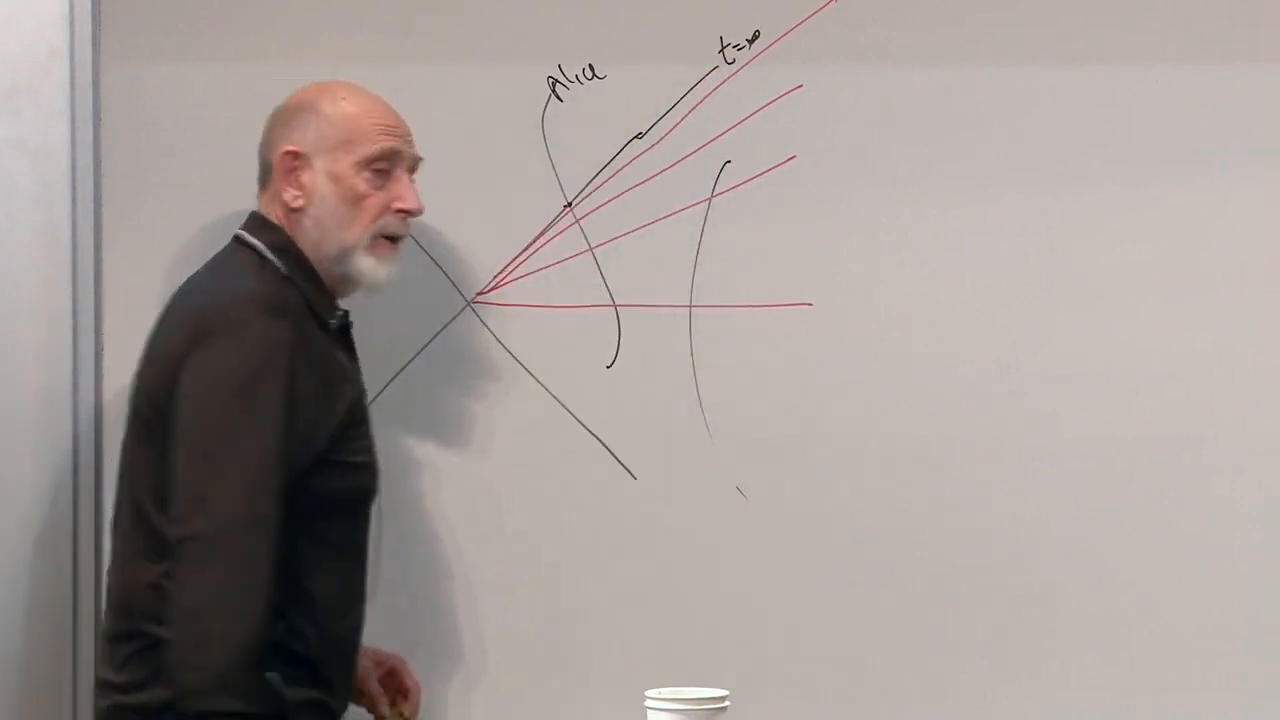
\includegraphics[width=0.84\textwidth]{lecture_07_figure_04.png}
\caption{Đường thế rơi vào của Alice và các tia có thời gian Schwarzschild không đổi. Tia giới hạn được gắn nhãn \(t=\infty\).}
\lectureframe{00:54:54}
\end{figure}

Alice rơi tự do. Đường thế của cô băng qua chân trời và chạm tới kỳ dị trong một thời gian riêng hữu hạn. Không có gì kỳ dị xảy ra với đồng hồ của cô tại chân trời nếu hố đen đủ lớn để lực thủy triều ở đó nhỏ.

Trái lại, Bob ở lại tại một bán kính ngoài cố định. Giữ nguyên vị trí đòi hỏi gia tốc. Ánh sáng từ những điểm muộn hơn trên đường thế của Alice đến chỗ anh sau những độ trễ ngày càng tăng và với độ dịch đỏ ngày càng lớn. Trong thời gian Schwarzschild, Alice tiệm cận \(t=\infty\) và Bob không bao giờ nhận được tín hiệu nào phát ra sau khi cô băng qua chân trời. Đó là những phát biểu về các tín hiệu nhân quả và phép lát cắt miền ngoài, chứ không phải bằng chứng cho một bề mặt vật chất tại chân trời.

\begin{classroomqa}
\audiencequestion{Nếu Bob thấy Alice chậm lại, thì Alice có nhất thiết phải thấy Bob nhanh lên không?}
\lecturerresponse{Không. Alice tiếp tục nhận các tín hiệu ánh sáng bình thường từ Bob chừng nào đường thế của cô còn kéo dài. Có một biến cố cuối cùng trên đường thế của Bob có thể đến được cô, nhưng biến cố đó là cuối cùng chỉ vì sau đó Alice đâm vào kỳ dị. Không có gì đột ngột xảy ra với Bob. Quan sát luôn nhìn vào một nón ánh sáng quá khứ, và hai đường thế có một quan hệ nhân quả bất đối xứng.
\lecturetimestamp{00:58:31--01:01:23}}
\end{classroomqa}

\begin{classroomqa}
\audiencequestion{Nếu Bob biết rằng trong các tọa độ của anh, Alice vẫn còn ở gần chân trời, liệu anh có thể đi xuống, cứu cô, rồi quay lại không?}
\lecturerresponse{Một đường thế cứu hộ phải gặp Alice trước khi cô băng qua chân trời sự kiện. Sau biến cố đó, không có đường đi hướng tương lai nào có thể gặp cô rồi quay trở lại bên ngoài. Việc các lát cắt Schwarzschild đặt lần băng qua tại \(t=\infty\) không có nghĩa là Alice ngồi lại trên một bề mặt vật chất có thể cứu ra được; nó cho thấy các lát cắt ấy không cung cấp một khái niệm toàn cục về “bây giờ” bắc qua chân trời.
\lecturetimestamp{01:01:24--01:02:12}}
\end{classroomqa}

\section{Charlie theo sau Alice}

Hãy để Charlie rơi cách sau Alice một đoạn ngắn. Khi đó cả hai đều xấp xỉ quán tính gần chân trời. Họ có thể trao đổi tín hiệu, trò chuyện theo cả hai hướng, hoặc thậm chí nắm tay nhau. Không ai gặp một cột mốc nào đánh dấu chân trời. Sự tương phản với Bob không phải là sự tương phản giữa ba người có tên riêng. Nó là sự tương phản giữa rơi tự do và một đường thế có gia tốc vẫn ở bên ngoài.

\begin{classroomqa}
\audiencequestion{Bob thấy gì nếu Alice rơi trước và Charlie theo sau, như một quả bóng rổ theo sau vành rổ?}
\lecturerresponse{Bob thấy cả hai cùng tiến lại gần chân trời. Alice, vì ở phía trước, là người trước hết có vẻ chậm dần đi và bị nén theo phương bán kính ngày càng nhiều. Charlie có vẻ ở càng lúc càng gần phía sau cô nhưng không bao giờ bắt kịp cô trong cái nhìn giới hạn từ bên ngoài của Bob. Sự dồn chồng về mặt hình ảnh đó không mô tả điều mà một trong hai người rơi vào cảm thấy.
\lecturetimestamp{01:04:12--01:06:05}}
\end{classroomqa}

\begin{classroomqa}
\audiencequestion{Sự dẹt đi biểu kiến có mâu thuẫn với lực thủy triều, vốn phải kéo giãn người rơi vào theo phương bán kính, hay không?}
\lecturerresponse{Đó là những hiệu ứng khác nhau. Sự dẹt đi thuộc về mô tả theo tọa độ Schwarzschild của Bob. Sự kéo dài do thủy triều là một hiệu ứng độ cong cục bộ mà Alice và Charlie có thể cảm nhận. Phần thảo luận về người quan sát giả thiết một hố đen đủ lớn, hoặc những người quan sát đủ nhỏ, để hiệu ứng thủy triều tại chân trời là không đáng kể. Trái lại, một hố đen cỡ khối lượng Mặt Trời sẽ có lực thủy triều ở chân trời dữ dội, còn một hố siêu khối lượng có thể có lực thủy triều ở chân trời yếu.
\lecturetimestamp{01:06:07--01:08:18}}
\end{classroomqa}

\begin{classroomqa}
\audiencequestion{Charlie có thấy Alice băng qua trong khi anh vẫn còn ở bên ngoài không?}
\lecturerresponse{Hãy vẽ tia null. Ánh sáng phát ra tại lúc Alice băng qua chạy dọc theo chân trời và tới Charlie khi Charlie băng qua. Tại biến cố đó, anh có thể tính ra rằng mình đã thấy cô băng qua, mặc dù cả hai người quan sát đều không gặp một dấu mốc cục bộ nào. Sau đó anh có thể thấy cô ở bên trong. Nếu anh gia tốc để đi ra xa trước khi băng qua và thành công trong việc vẫn ở bên ngoài, thì anh không bao giờ thấy lần băng qua ấy.
\lecturetimestamp{01:08:19--01:11:11}}
\end{classroomqa}

\begin{classroomqa}
\audiencequestion{Nếu Alice đã ở bên trong còn Charlie ở bên ngoài, thì làm sao có thể so sánh các bán kính về sau và các thời điểm băng qua của họ?}
\lecturerresponse{Không có một quan hệ đồng thời nào độc lập với người quan sát để có thể đọc ra từ một cụm như “cùng một lúc”. Alice thấy Charlie trên nón ánh sáng quá khứ của mình và chỉ có thể thấy lần băng qua muộn hơn của anh khi cô đã vào sâu hơn bên trong. Chính các đường thế và các tia null cụ thể mới trả lời câu hỏi. Một ngoại suy rộng cho nhiều người rơi vào cách xa nhau phải được kiểm tra bằng cách vẽ giản đồ nhân quả thực sự của họ thay vì giả sử có một thời điểm băng qua phổ quát.
\lecturetimestamp{01:11:14--01:12:31}}
\end{classroomqa}

Trong các tọa độ chính quy gần chân trời, một quỹ đạo rơi tự do gần như là một đường thẳng. Nó không hoàn toàn thẳng trong hình học Schwarzschild đầy đủ, nhưng phép gần đúng trở nên tốt gần một chân trời lớn, có độ cong yếu.

\begin{classroomqa}
\audiencequestion{Liệu lý thuyết dây có thể giải quyết điều gì xảy ra trong chế độ hấp dẫn lượng tử ở phần bên trong hố đen không?}
\lecturerresponse{Đó chính là nơi chủ đề này trở nên tinh tế. Cần có một lý thuyết hấp dẫn lượng tử gần kỳ dị, và lý thuyết dây là một khuôn khổ ứng viên, nhưng các câu hỏi liên quan khi ấy vẫn là những câu hỏi đang được nghiên cứu và khó khăn, chứ không được giải quyết bằng một áp dụng đơn giản của giản đồ cổ điển.
\lecturetimestamp{01:13:04--01:13:38}}
\end{classroomqa}

\begin{classroomqa}
\audiencequestion{Điều gì xảy ra với đồng hồ và vận tốc của chính Alice khi cô băng qua?}
\lecturerresponse{Đồng hồ của cô tiếp tục chạy theo tốc độ cục bộ thông thường của nó và ghi lại một thời gian riêng hữu hạn. Trong hệ quy chiếu nghỉ tức thời của mình, cô đứng yên; so với một hệ rơi tự do cục bộ, cô có một vận tốc hữu hạn bình thường. Gần một chân trời lớn, hình học gần như phẳng, nên các mốc thời gian riêng bằng nhau dọc theo đường thế của cô vẫn đều đặn cho đến khi độ cong trở nên mạnh gần kỳ dị.
\lecturetimestamp{01:13:39--01:14:44}}
\end{classroomqa}

\begin{classroomqa}
\audiencequestion{Nếu Bob gia tốc ra ngoài nhưng không đủ mạnh để tránh rơi xuyên qua thì sao?}
\lecturerresponse{Khi đó đường thế của anh cong ra ngoài nhưng vẫn băng qua chân trời. Nếu anh băng qua rất muộn, anh có thể thấy Alice không lâu sau lần băng qua của cô, nhưng thời gian riêng còn lại của anh trước khi tới kỳ dị thì ngắn. Độ dốc của các đường thế trên hình phác không phải là những thước đo hay đồng hồ đã hiệu chuẩn; điều còn lại là thứ tự nhân quả, chứ không phải các độ dài Euclid được vẽ của chúng.
\lecturetimestamp{01:14:47--01:16:31}}
\end{classroomqa}

Tất cả các kết luận này đều giả thiết rằng không tín hiệu nào vượt ánh sáng. Bài giảng thoáng đùa về các bản tin báo chí mới đây khi đó nói đến những neutrino dường như siêu quang ở Ý, một ám chỉ đến lỗi định thời thí nghiệm chứ không phải một ngoại lệ đối với thuyết tương đối. Bản thân cách dựng nhân quả vẫn bị chặn bởi các đường null.

\begin{classroomqa}
\audiencequestion{Liệu những đồng hồ đã được đồng bộ mà Alice và Bob mang theo có thể phân xử câu hỏi ấy nếu Alice lao về phía chân trời rồi quay lại không?}
\lecturerresponse{Họ có thể so sánh đồng hồ khi họ trùng nhau, nhưng sau khi các đường thế của họ tách ra thì không có một sự đồng bộ từ xa duy nhất nào, đặc biệt khi một người thay đổi chuyển động. Hãy vẽ cả hai đường thế và các tia null được trao đổi. Giản đồ đó cung cấp câu trả lời thao tác cho bất kỳ thí nghiệm nào được nêu rõ.
\lecturetimestamp{01:17:34--01:18:25}}
\end{classroomqa}

\begin{figure}[htbp]
\centering
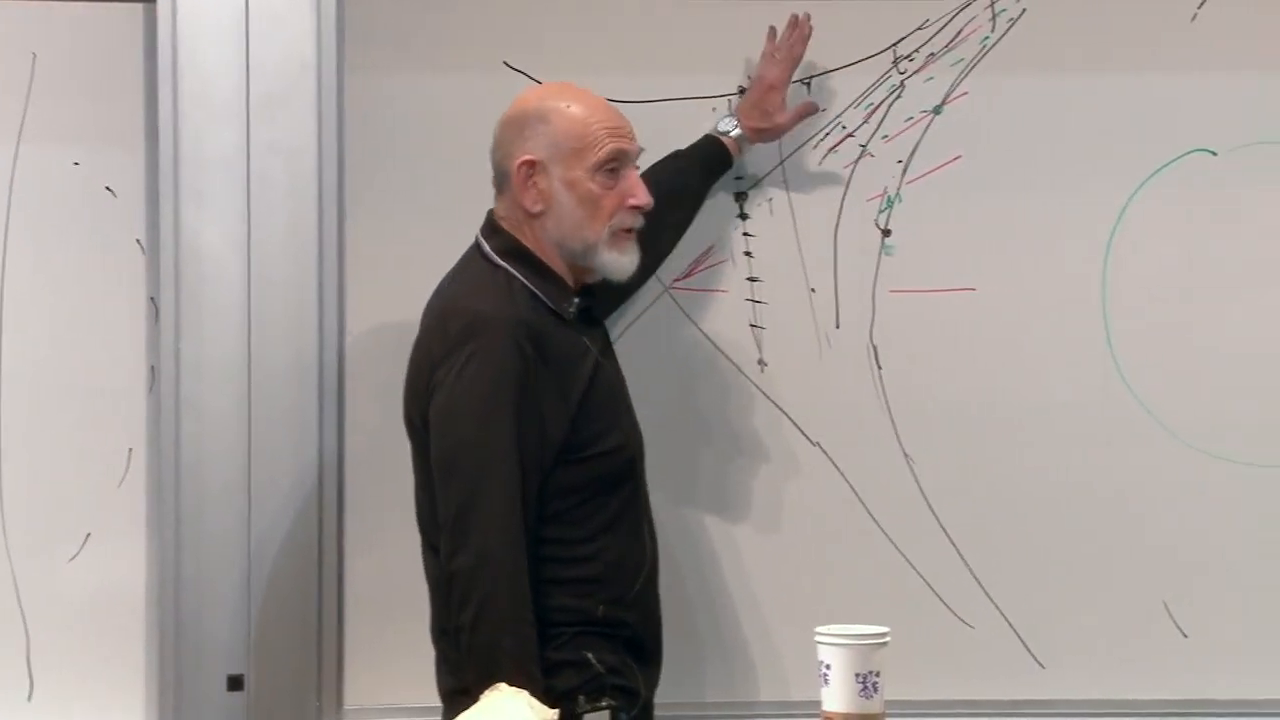
\includegraphics[width=0.86\textwidth]{lecture_07_figure_05.png}
\caption{Giản đồ nhân quả tổng hợp được dùng để trả lời các câu hỏi về Alice, Bob và Charlie. Mỗi quan sát được định vị bằng cách truy vết một tia null từ biến cố được quan sát tới đường thế của người quan sát.}
\lectureframe{01:18:12}
\end{figure}

\begin{figure}[htbp]
\centering
\resizebox{0.96\linewidth}{!}{%
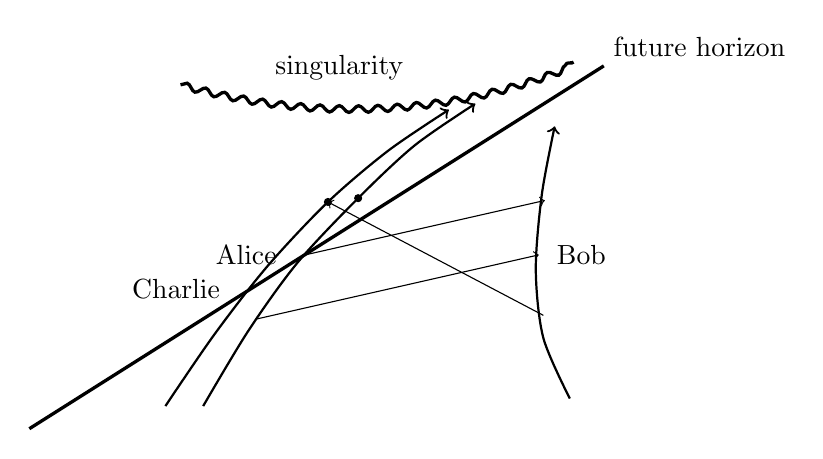
\begin{tikzpicture}[scale=0.96]
\draw[very thick] (-3.8,-0.3) -- (3.8,4.5);
\node[above right] at (3.8,4.5) {future horizon};
\draw[very thick,decorate,decoration={snake,amplitude=1.2pt,segment length=7pt}]
  (-1.8,4.25) .. controls (0.1,3.72) and (2.0,3.92) .. (3.4,4.55);
\node at (0.3,4.48) {singularity};
\draw[thick,->]
  plot[smooth] coordinates {(-1.5,0.0) (-0.9,1.0) (-0.25,1.9)
  (0.55,2.75) (1.3,3.45) (2.1,4.0)};
\node[left] at (-0.4,2.0) {Alice};
\draw[thick,->]
  plot[smooth] coordinates {(-2.0,0.0) (-1.35,0.95) (-0.65,1.85)
  (0.15,2.7) (0.95,3.38) (1.75,3.92)};
\node[left] at (-1.15,1.55) {Charlie};
\draw[thick,->]
  plot[smooth] coordinates {(3.35,0.1) (3.0,0.9) (2.9,1.8)
  (2.98,2.8) (3.15,3.7)};
\node[right] at (3.05,2.0) {Bob};
\draw[thin,->] (-0.8,1.15) -- (2.94,2.0);
\draw[thin,->] (-0.15,2.0) -- (3.02,2.72);
\draw[thin,->] (3.0,1.2) -- (0.15,2.7);
\draw[fill] (0.55,2.75) circle (1.3pt);
\draw[fill] (0.15,2.7) circle (1.3pt);
\end{tikzpicture}
}
\caption{Một giản đồ phác họa về người quan sát. Các quan sát bên ngoài của Bob và các quan sát lẫn nhau của Alice và Charlie là những cách dựng bằng tia null khác nhau, chứ không phải những khẩu hiệu đối ứng về đồng hồ.}
\label{fig:l7-observers-clean}
\end{figure}

\begin{classroomqa}
\audiencequestion{Bob có nhìn thấy Alice trong một thời gian vô hạn không, và điều đó có nghĩa là trong thực tại của anh ấy cô ấy không bao giờ chết sao?}
\lecturerresponse{Bob nhận được các tín hiệu của cô ấy trong một khoảng thời gian không bị chặn theo thời gian của chính anh ấy, nhưng anh ấy thấy đồng hồ của cô ấy chậm dần tới tốc độ 0 và chỉ nhận được chuỗi nhịp tim hữu hạn được phát ra trước khi cô ấy băng qua. Từ “thực tại” che khuất sự phân biệt giữa một sự kiện cục bộ và bản ghi tiệm cận của một người quan sát. Alice không hề trải qua một chiếc đồng hồ bị dừng lại ở chân trời; bản ghi của Bob ngày càng bị trễ và bị dịch đỏ.
\lecturetimestamp{01:18:32--01:20:59}}
\end{classroomqa}

\begin{classroomqa}
\audiencequestion{Sau khi băng qua, Alice có đột nhiên nhìn thấy toàn bộ vật chất từ trước vốn có vẻ bị đóng băng trên chân trời không?}
\lecturerresponse{Không có chuyện bỗng nhiên mọi thứ trở nên rõ ràng. Khi rơi vào, các nón ánh sáng quá khứ qua đó cô ấy nhìn thấy vật chất trước đó thay đổi một cách liên tục. Cô ấy có thể suy ra rằng ánh sáng đang tới chỗ mình bây giờ đã được phát ra sớm hơn và rằng vật chất ấy đã băng qua trước cô ấy. Cách Charlie quan sát Alice cho thấy cùng một điều: không có lần băng qua nào tạo ra một gián đoạn cục bộ hay để lộ ra một đống ghế và khủng long bị che giấu.
\lecturetimestamp{01:21:02--01:23:48}}
\end{classroomqa}

\begin{classroomqa}
\audiencequestion{Có những mô phỏng hiện thực về những gì một người rơi vào sẽ nhìn thấy không?}
\lecturerresponse{Bài giảng chỉ đến các mô phỏng trực quan hóa lỗ đen của Andrew Hamilton. Chúng có thể truyền đạt được quang sai mạnh và các dịch chuyển tần số của ánh sáng đi tới, mặc dù phần hiển thị có thể gây mất phương hướng nhiều hơn là làm sáng tỏ. “Không có gì đặc biệt ở chân trời” nói về hình học cục bộ, chứ không phải về một bầu trời trông bình thường.
\lecturetimestamp{01:24:11--01:25:29}}
\end{classroomqa}

\section{Từ lỗ đen vĩnh cửu đến lỗ đen đang lớn dần}

Đỉnh dưới của giản đồ vĩnh cửu được mở rộng tối đại có rất ít ý nghĩa trực tiếp đối với một lỗ đen được hình thành do sự suy sụp sao. Chỉ phần chứa miền ngoài, chân trời tương lai và miền trong tương lai mới xuất hiện trong hình học suy sụp đơn giản. Sự phân biệt này trở nên thiết yếu khi cho phép vật chất làm thay đổi khối lượng của lỗ đen.

\begin{classroomqa}
\audiencequestion{Sự kiện vật lý nào được biểu diễn bởi đỉnh dưới của giản đồ lý tưởng hóa?}
\lecturerresponse{Đối với nghiệm toán học vĩnh cửu, nó là một phần của phần mở rộng tối đại. Một lỗ đen hình thành từ vật chất suy sụp không chứa toàn bộ vùng dưới ấy. Chân trời của nó có một lịch sử hình thành, điều này đòi hỏi một giản đồ toàn cục khác và sẽ được phát triển trong bài giảng tiếp theo.
\lecturetimestamp{01:25:59--01:26:52}}
\end{classroomqa}

Khi một vật thử nhỏ rơi vào, có thể bỏ qua phản hồi ngược của nó và giản đồ Schwarzschild cố định là đủ dùng. Nếu một khối lượng đáng kể rơi vào, khối lượng của lỗ đen và bán kính Schwarzschild tăng lên:
\begin{equation}
r_{\mathrm S}=2GM,
\qquad
\Delta r_{\mathrm S}=2G\,\Delta M.
\label{eq:l7-growing-radius}
\end{equation}
Chân trời biến dạng về phía vật đang đi vào, các chân trời nhập lại, và chân trời chung bị méo nhanh chóng lắng xuống. Trong lý tưởng hóa không quay của bài giảng, trạng thái cuối là một mặt cầu lớn hơn đôi chút. Một vụ sáp nhập thực cũng bức xạ năng lượng dưới dạng sóng hấp dẫn và nói chung để lại một lỗ đen quay.

\begin{classroomqa}
\audiencequestion{Nếu chân trời lớn ra khi khối lượng rơi vào, liệu nó có dịch ra ngoài để gặp vật chất dường như bị đóng băng gần chân trời cũ không?}
\lecturerresponse{Đối với một vật đang rơi vào có khối lượng đủ lớn, bức tranh hạt thử không còn đúng nữa. Chân trời biến dạng, nhập với miền bị bẫy của vật đang đi vào, rồi lắng về một chân trời dừng lớn hơn. Việc xác định chính xác vị trí của chân trời sự kiện là một bài toán toàn cục và nó có thể kéo dài vào một vùng từ trước khi vật chất rơi vào tới nơi. Bài giảng cố ý hoãn việc xây dựng đầy đủ sang buổi học tiếp theo.
\lecturetimestamp{01:26:55--01:29:05}}
\end{classroomqa}

\begin{classroomqa}
\audiencequestion{Tại sao các nhà thiên văn học có thể quan sát các chớp sáng khi vật chất được cho là cần thời gian Schwarzschild vô hạn để tới chân trời?}
\lecturerresponse{Bức xạ sáng không phát ra từ chính chân trời. Khí trong dòng bồi tụ hoặc đĩa bồi tụ va chạm và nóng lên ở bên ngoài chân trời, kể cả gần các quỹ đạo photon mạnh. Plasma ở bên ngoài đó có thể phát ra ánh sáng truyền tới chúng ta. Hình học Schwarzschild chân không tách riêng vấn đề nhân quả nhưng không phải là một mô hình hoàn chỉnh của môi trường vật lý thiên văn.
\lecturetimestamp{01:29:07--01:30:22}}
\end{classroomqa}

Thời gian thư giãn đặc trưng được xác định bởi thời gian ánh sáng đi ngang qua:
\begin{equation}
t_{\mathrm{cross}}\sim\frac{r_{\mathrm S}}{c},
\qquad
t_{\mathrm{relax}}\sim
\text{a few to a few tens of }t_{\mathrm{cross}}.
\label{eq:l7-relaxation-scale}
\end{equation}
Bài giảng ước tính \(10^{-5}\,\mathrm{s}\) là thời gian đi ngang qua của một lỗ đen cỡ kilômét và xấp xỉ \(10^{-3}\,\mathrm{s}\) để một vụ sáp nhập nhỏ trở nên gần như dừng. Đối với một lỗ đen khối lượng một tỷ khối lượng Mặt Trời, thời gian tương ứng được tính bằng phút đến giờ. Đây là các ước lượng theo luật tỉ lệ, không phải các phép tính sáp nhập chính xác. Điểm cốt yếu là chuỗi hình học: hình quả tạ, hình hạt lạc, gần như hình cầu, dừng.

\begin{classroomqa}
\audiencequestion{Một chân trời bị méo hoặc vừa sáp nhập sẽ lắng xuống nhanh đến mức nào?}
\lecturerresponse{Trên một thang thời gian không dài hơn quá nhiều so với thời gian ánh sáng cần để đi qua lỗ đen. Vì mọi độ dài và thời gian đều tỉ lệ với \(r_{\mathrm S}\), các lỗ đen nhỏ lắng xuống trong những phần của một giây còn các lỗ đen siêu khối lượng lớn thì trên các thời gian đồng hồ dài hơn nhiều. Phát biểu không tóc mô tả trạng thái cuối dừng; biến dạng quá độ mang năng lượng đi dưới dạng bức xạ hấp dẫn.
\lecturetimestamp{01:30:26--01:33:18}}
\end{classroomqa}

\begin{classroomqa}
\audiencequestion{Bob nhìn thấy gì nếu vật chất từ trước nằm giữa chân trời cũ và chân trời mới trong khi một vật thể nặng khác rơi vào?}
\lecturerresponse{Câu hỏi đó không thể được trả lời một cách nhất quán bằng cách vá hai giản đồ Schwarzschild tĩnh lại với nhau. Cần phải giải hoặc dựng hình học suy sụp phụ thuộc thời gian và xác định chân trời toàn cục của nó. Bài giảng giữ lại câu hỏi này và nói rõ rằng câu trả lời sẽ được hoãn đến tuần sau, khi sự hình thành chân trời là chủ đề của buổi học.
\lecturetimestamp{01:33:20--01:35:41}}
\end{classroomqa}

\section{Điều gì thay đổi khi quy mô thay đổi?}

Giản đồ không thứ nguyên không thay đổi khi \(r_{\mathrm S}\) thay đổi. Còn ý nghĩa vật lý của một đoạn được vẽ thì có thay đổi:
\begin{equation}
d\tau_{\mathrm{physical}}^2
=
r_{\mathrm S}^2\,d\hat{\tau}^2,
\qquad
\ell_{\mathrm{physical}}
=
r_{\mathrm S}\,\hat{\ell}.
\label{eq:l7-scale-restoration}
\end{equation}
Một độ tách không thứ nguyên biểu diễn nửa kilômét đối với một lỗ đen cỡ kilômét sẽ biểu diễn xấp xỉ nửa tỷ kilômét đối với một lỗ đen lớn hơn một tỷ lần. Phép tương tự với các hình cầu được vẽ giống hệt nhau lại quay trở lại: hình dạng không đổi, còn số thước mét mà một đoạn thẳng biểu diễn thì tỉ lệ với bán kính.

\begin{classroomqa}
\audiencequestion{Giản đồ nhân quả thay đổi như thế nào khi bán kính Schwarzschild thay đổi?}
\lecturerresponse{Nó không thay đổi sau khi đã chuẩn hoá để khử bán kính đó. Mọi độ dài và thời gian vật lý gán cho giản đồ đều được nhân với \(r_{\mathrm S}\), trong khi độ cong tại các điểm không thứ nguyên tương ứng được nhân với \(r_{\mathrm S}^{-2}\).
\lecturetimestamp{01:35:41--01:38:10}}
\end{classroomqa}

\begin{classroomqa}
\audiencequestion{Kết luận nhân quả có thay đổi không nếu Bob chuyển động trên quỹ đạo thay vì lơ lửng tại một vị trí góc cố định?}
\lecturerresponse{Các dịch đỏ chi tiết và các hướng tới trở nên phức tạp hơn, nhưng sự tách biệt nhân quả của chân trời không thay đổi. Không một quỹ đạo kiểu thời nào ở miền ngoài nhận được tín hiệu phát ra từ bên trong chân trời.
\lecturetimestamp{01:38:12--01:38:26}}
\end{classroomqa}

\begin{classroomqa}
\audiencequestion{Vì lực hấp dẫn triệt tiêu bên trong một vỏ cầu, liệu nó có triệt tiêu bên trong chân trời vì khối lượng của lỗ đen được phân bố trên bề mặt ấy không?}
\lecturerresponse{Không. Chân trời sự kiện không phải là một vỏ vật chất mang khối lượng. Vì thế định lý vỏ cầu Newton không áp dụng cho nó. Bài giảng so sánh nghiệm ngoài tĩnh với một nguồn điểm tại kỳ dị độ cong, nhưng vật chất đang rơi vào trong quá trình hình thành đòi hỏi hình học phụ thuộc thời gian, vốn được hoãn sang bài giảng tiếp theo.
\lecturetimestamp{01:38:28--01:40:41}}
\end{classroomqa}

\section{Sự quay và hình học theo phương bán kính}

Mômen động lượng vẫn tồn tại qua sự suy sụp. Một lỗ đen quay có hình học bên ngoài khác với Schwarzschild: nghiệm dừng của nó là Kerr, sự quay làm méo hình học chân trời, và hiệu ứng kéo hệ quy chiếu kéo các phương quán tính xoay quanh lỗ đen. Về nguyên tắc, mômen động lượng được đo từ các hiệu ứng hấp dẫn bên ngoài đó. Vật chất có mômen động lượng không mất nó chỉ vì băng qua một chân trời.

\begin{classroomqa}
\audiencequestion{Lỗ đen có thể có mômen động lượng đo được không, và sự quay có làm thay đổi hấp dẫn ở bên ngoài nó không?}
\lecturerresponse{Có. Mômen động lượng vẫn còn như một tham số bảo toàn, làm biến dạng hình học dừng và sinh ra hiệu ứng kéo hệ quy chiếu. Chân trời khi ấy không còn là chân trời Schwarzschild hình cầu đơn giản nữa. Bài giảng so sánh một cách định tính sự biến dạng ấy với dạng dẹt của Trái Đất, đồng thời lưu ý rằng nghiệm quay đầy đủ phức tạp hơn đáng kể.
\lecturetimestamp{01:40:45--01:42:36}}
\end{classroomqa}

\begin{classroomqa}
\audiencequestion{Liệu quan hệ giữa \(r\) và khoảng cách riêng \(\rho\) có nghĩa là hấp dẫn làm co không gian không?}
\lecturerresponse{Khoảng cách riêng theo phương bán kính \(\rho\) thỏa mãn \begin{equation*}
\frac{d\rho}{dr}=\sqrt{\frac{r}{r-1}}>1
\end{equation*} bên ngoài chân trời đơn vị. Vì vậy, một độ tăng tọa độ \(dr\) cho trước tương ứng với một khoảng riêng theo phương bán kính lớn hơn ở gần chân trời. Việc nói không gian bị co hay bị giãn phụ thuộc vào những khoảng tọa độ nào đang được đem so sánh. Phát biểu bất biến chính là bản thân quan hệ khoảng cách riêng ấy.
\lecturetimestamp{01:42:36--01:43:20}}
\end{classroomqa}

\section{Câu hỏi cuối cùng}

\begin{classroomqa}
\audiencequestion{Theo cách nhìn của Bob, đồng hồ của Alice tiến gần tới chỗ ngừng chạy. Theo cách nhìn của Alice, không gian hay thời gian của Bob có kết thúc không?}
\lecturerresponse{Không. Alice nhìn thấy những tín hiệu bình thường từ các sự kiện liên tiếp trên đường thế giới của Bob cho đến khi chính đường thế giới của cô kết thúc. Cô không thấy các sự kiện muộn hơn của Bob vì không tồn tại điểm nào muộn hơn trên đường thế giới của cô, chứ không phải vì Bob hay không gian của anh biến mất. Trong các tọa độ nhân quả chính quy này, các tia không xuyên tâm được vẽ thành đường thẳng; việc chúng hiện ra như những quỹ đạo cong trong một hệ tọa độ khác không làm thay đổi những sự kiện mà chúng nối với nhau.
\lecturetimestamp{01:43:21--01:45:20}}
\end{classroomqa}

Thuyết tương đối rộng đặt ra hai nhiệm vụ bổ sung cho nhau. Với một metric đã cho, ta có thể lần theo các đường trắc địa và các tia không để xác định những gì các quan sát viên đo được. Với một phân bố vật chất đã cho, ta phải giải các phương trình Einstein để tìm metric. Nhiệm vụ thứ nhất đã chiếm phần lớn bài giảng này. Nhiệm vụ thứ hai thường khó hơn, mặc dù sự suy sụp đối xứng cung cấp những ví dụ còn có thể xử lý được.

\begin{classroomqa}
\audiencequestion{Điều gì xảy ra với chân trời và kỳ dị của một lỗ đen đang bay hơi?}
\lecturerresponse{Bài giảng đưa ra một bức tranh sơ đồ trong đó chân trời co lại và gặp điểm cuối của vùng kỳ dị. Sự bay hơi là một quá trình lượng tử bán cổ điển, và điểm cuối ở thang Planck không được quyết định bởi biểu đồ Schwarzschild cổ điển. Vì vậy, hình phác co nhỏ ấy nên được hiểu như một sự xem trước định tính, chứ không phải một hình học lượng tử hoàn chỉnh.
\lecturetimestamp{01:46:04--01:46:32}}
\end{classroomqa}

Hầu như mọi lỗ đen thiên văn đều phải quay. Các ngôi sao vốn đã mang mômen động lượng, và sự suy sụp làm tăng vận tốc góc của chúng theo cách quen thuộc như một vận động viên trượt băng khép tay vào người. Cấu trúc kỳ dị của một lỗ đen Kerr không phải là mặt Schwarzschild \(r=0\) được vẽ ở đây, và không nên mô tả nó như thể vật chất thực sự quay với tốc độ tuyến tính vô hạn.

\begin{classroomqa}
\audiencequestion{Các lỗ đen vĩ mô không quay có phổ biến không, và có bao nhiêu lỗ đen?}
\lecturerresponse{Mômen động lượng đúng bằng không sẽ là một sự lý tưởng hóa rất đặc biệt. Bài giảng chỉ đưa ra một ước lượng bậc độ lớn kiểu trên lớp cho quần thể trong vũ trụ, nằm đâu đó giữa số lượng thiên hà và số lượng sao, và có lẽ vào khoảng \(10^{15}\). Đó là một ước lượng vào thời điểm của bài giảng, không phải một cuộc kiểm kê đã được đo đạc. Điểm chắc chắn là sự suy sụp nhìn chung bảo toàn và khuếch đại một phần mômen động lượng.
\lecturetimestamp{01:46:32--01:48:42}}
\end{classroomqa}

\begin{classroomqa}
\audiencequestion{Lỗ đen hình thành từ vật chất có sẵn hay xuất hiện thông qua một quá trình lượng tử?}
\lecturerresponse{Các lỗ đen thiên văn thông thường hình thành khi vật chất sao có sẵn suy sụp. Sự cháy hạt nhân và dòng năng lượng hướng ra ngoài giúp nâng đỡ một ngôi sao. Khi nhiên liệu cạn kiệt, tàn dư co lại. Tùy theo khối lượng của nó và lực đỡ áp suất sẵn có, nó có thể trở thành một sao lùn trắng, một sao neutron, hoặc, nếu không có lực đỡ nào có thể chặn sự suy sụp, đi vào bên trong bán kính Schwarzschild của chính nó và hình thành một lỗ đen.
\lecturetimestamp{01:48:43--01:50:23}}
\end{classroomqa}

\begin{classroomqa}
\audiencequestion{Các lỗ đen vi mô có thể hình thành không, và điều gì sẽ quyết định thời gian sống và kích thước tối thiểu của chúng?}
\lecturerresponse{Phần này mang tính suy đoán. Sự bay hơi Hawking diễn ra nhanh hơn đối với khối lượng nhỏ hơn, với thời gian sống tỷ lệ gần đúng như \(M^3\). Bài giảng dùng phép so sánh với khối lượng cỡ một ngọn núi cho một lỗ có thời gian sống có thể ở thang vũ trụ học; phép so sánh bằng số ấy chỉ là gần đúng thô. Những thăng giáng mật độ dữ dội trong vũ trụ sơ khai hoặc những va chạm đủ năng lượng là các cơ chế hình thành có thể hình dung được. Một lỗ đen gần khối lượng Planck, xấp xỉ \(10^{-5}\,\mathrm{g}\), đánh dấu thang mà tại đó một mô tả hình học cổ điển không còn đáng tin cậy. Để đạt tới năng lượng đó trong một máy gia tốc thông thường sẽ cần một cỗ máy lớn đến mức khó tin nếu ngoại suy một cách trực tiếp, mặc dù về nguyên tắc sự hình thành như vậy là có thể.
\lecturetimestamp{01:50:23--01:53:31}}
\end{classroomqa}

\begin{classroomqa}
\audiencequestion{Khóa học này có kịp đi tới vũ trụ học, vật chất tối, năng lượng tối, entropy và sóng hấp dẫn không?}
\lecturerresponse{Các ứng dụng vũ trụ học, và có lẽ cả sóng hấp dẫn, vẫn có thể là những chủ đề về sau. Entropy của lỗ đen được hoãn sang sau quý học này. Bài giảng khép lại bằng việc chấp nhận rằng tối hôm đó chỉ trình bày được khoảng một phần tư nội dung đã dự kiến: giải quyết các câu hỏi một cách cẩn trọng quan trọng hơn là lao nhanh qua dàn ý.
\lecturetimestamp{01:53:33--01:54:38}}
\end{classroomqa}

Quy tắc thao tác ấy vẫn đứng vững trước mọi câu hỏi trong phòng học. Hãy chỉ rõ các đường thế giới, vẽ các tia không, và xác định các sự kiện mà chúng nối với nhau. Chân trời không phải là nơi mà vật lý địa phương mất hiệu lực; nó là ranh giới mà một khi vượt qua nó, mọi tín hiệu hướng về tương lai đều vẫn ở bên trong. Bài giảng tiếp theo thay bối cảnh vĩnh cửu bằng một nguồn đang suy sụp và cho thấy ranh giới ấy được hình thành như thế nào.